\documentclass{article}

\usepackage{amsmath} % Used for mathematical formulas
\usepackage{graphicx} % Used for inserting images
\usepackage{lipsum} % Used for generating placeholder text
\usepackage{ctex} % Imported the ctex package to support Chinese
% \usepackage{titlesec} % Imported the titlesec package for customizing title styles
% \usepackage{fontspec} % Used for setting Chinese fonts

% \setmainfont{SimSun} % Set the Chinese font to SimSun (宋体 system font)

\usepackage{listings}
\usepackage{color}
\usepackage{float}

\title{基于LLM的选课管理系统项目开发方案}
\author{程智镝,汪天佑,陈凌,刘辉}
\date{\today}

\begin{document}
\maketitle

% 添加目录
\tableofcontents

\newpage

\section{项目概述}

\subsection{项目名称}
基于LLM的选课管理系统

\subsection{项目目标}
开发一个基于自然语言处理技术的在线选课管理系统,为学生和教务管理人员提供高效、智能的选课服务。

\subsection{项目团队}
刘  辉 211250122,程智镝 211250124,陈  凌 211250159,汪天佑 211250173

\subsection{项目背景}
\begin{itemize}
	\item 学校选课管理需求:随着招生的扩大和课程数量的增加,传统的选课管理方式已经无法满足学生和教务管理人员的需求。通过引入先进的LLM技术,改进选课管理流程,提高选课效率和质量。
	\item LLM技术的发展:随着自然语言处理技术的发展,利用这项技术来构建智能化的选课管理系统,将能够提高系统的智能程度,增强用户体验。
\end{itemize}

\section{关键问题}
\subsection{项目吸引力问题}
\begin{itemize}
	\item 项目的吸引力在哪里?\\
	1.创新性:我们的系统创新性地结合了LLM技术,能够提供更智能、个性化的选课建议和服务,帮助学生更快速、更准确地选择适合自己的课程。\\
	2.实用性:我们的系统致力于解决在效率低、用户体验差等问题,提供简洁易用的界面、智能化的选课推荐功能以及快速高效的选课流程,提高选课的便捷性和效率性。\\
	\item 如何令评审专家满意?\\
	为了使得评审专家满意,我们致力于做到以下几点:\\
	1.详细的项目规划和时间安排:我们将提供清晰明确的项目计划,包括开发阶段、里程碑和交付时间,以展现我们的组织能力和执行力。(详情见 5.开发计划)\\
	2.丰富的功能:我们通过引入LLM技术,致力于为师生提供具有丰富、便捷的功能的选课系统。(详情见 6.功能特点)\\
	3.优秀的用户体验设计:我们将注重用户体验,使用 Ant Design Vue 等现代前端开发库,设计直观友好的界面,确保教务方面和学生能够轻松快捷地完成排课、选课操作,并提供全方位的技术支持和用户培训,以确保用户满意度。(详情见 7.用户体验和界面设计)\\
	4.可靠的质量和后续服务:我们将使用 JUnit 和 Mockito 等工具进行测试,执行质量保障环节,建立完善的技术支持体系,提供持续的系统维护和升级服务,保障系统的稳定性和可靠性。(详情见 8.测试和质量保证,及 9.部署和维护)\\
\end{itemize}

\subsection{项目执行问题}
\begin{itemize}
	\item 能否完成任务?\\
	我们的团队拥有丰富的开发经验和成熟的技术实力,具备完成该项目的能力。我们将充分利用团队成员的专业技能和资源,制定明确的项目计划,确保项目按时交付并达到预期目标。
	\item 如何控制项目的进度?\\
	为了控制项目的进度,我们将采取以下措施:\\
	1.制定详细的项目计划,根据实际需要对具体任务进行详细的描述。(详情见 5.开发计划)\\
	2.持续跟踪和监控:我们将定期进行项目进度的跟踪和监控,及时发现和解决可能影响项目进度的问题,并及时调整计划以保证项目的顺利进行。\\
	3.沟通与协作:我们将建立高效的沟通机制,确保团队成员之间的信息流畅和协作顺畅,以提高工作效率和项目执行速度。\\
	\item 产品的质量如何保证?\\
	我们有严格确保产品质量的要求(详情见 8.测试和质量保证)
	\item 产品的成本如何控制?\\
	我们会对预算和所需资源进行评估,确保项目成本在预期之内(详情见 10.预算和资源)
\end{itemize}

\subsection{团队能力和信任问题}
\begin{itemize}
	\item 如何让别人相信团队能完成任务?\\
	1.我们的团队将向客户展示我们以往的项目、作品以及客户推荐信等,以此证明我们团队的实力
	2.我们将分析、度量项目的规模,给出详细的项目工作计划,让客户对我们的工作有信心
	\item 团队的工作计划是什么样的?\\
	详情请见 5.开发计划
	\item 如何让人相信这个计划可行?\\
	1.我们的计划将对项目进行度量,提高客户对此计划可行性的信任度
	2.我们的计划纳入了各项风险评估和应对策略,使用户不必担心风险造成的项目失败
\end{itemize}

\subsection{风险管理}
\begin{itemize}
	\item 项目有哪些潜在风险?\\
	项目可能存在技术风险、安全风险、人员风险、范围风险、时间风险、资源风险、性能风险、管理风险等风险
	\item 如何应对风险?\\
	我们有详细的风险应对策略。我们对技术、管理和资源风险进行详细的描述,并提供了具体的应对策略。(详情见 5.2 项目风险管理)\\
	我们还会使用 Log4j2 进行日志和监控。
\end{itemize}

\subsection{用户体验和反馈问题}
\begin{itemize}
	\item 项目如何提高用户体验?\\
	我们为用户设计了良好的交互(详情见 7.1 用户友好的界面设计原则,7.2 屏幕原型)
	\item 项目将如何收集用户反馈并改进?\\
	我们为用户提供了反馈渠道,并制定了一套改进计划(详情见7.3 用户反馈和改进计划)
\end{itemize}

\subsection{部署和维护问题}
\begin{itemize}
	\item 项目是否有部署计划?\\
	我们为项目制定了部署计划(详情见 9.1 部署计划)
	\item 项目将如何维护?\\
	我们的项目具有日常维护计划和版本升级计划,确保项目的正常运作(详情见 9.2 维护策略)
\end{itemize}

\section{需求分析}
\subsection{需求规格说明描述}
\paragraph{系统基本特性}
\begin{itemize}
	\item \textbf{系统类型:} 基于WEB的选课管理系统。
	\item \textbf{用户角色:} 学生、管理员。
	\item \textbf{用户登录和身份验证要求:} 用户需通过用户名和密码进行登录验证。
	\item \textbf{邮件支持:} 系统支持通过电子邮件发送选课通知、选课结果等信息至学生邮箱(软件学院),并支持用户注册、密码取回等功能。
\end{itemize}

\paragraph{邮件支持}
\begin{itemize}
	\item \textbf{邮件通知:} 可以发送选课通知、选课结果等信息至学生邮箱(软件学院)。
	\item \textbf{邮件验证:} 用户注册、密码取回等也可以通过邮件发送。
\end{itemize}

\paragraph{以院系为单位支持管理功能}
\begin{itemize}
	\item \textbf{支持导入、保存和修改课程计划:} 导入的格式由excel 模板给出,该模板可以下载。
	\item \textbf{支持管理员对课程进行设置:} 管理员可以设置选课人数上限、先修课程限制、选课者年级(不允许提前两个学年选课),以及设定课程的性质、介绍信息、课程目标、课程内容、教材、考试方式 等
	\item \textbf{其他课程设置要求}
	(1) 对每个学生,管理员可设定可选课程数量上限和必选课程数量下限\\
	(2) 设定选课期限,在期限内可以选课,超出期限则不能选课\\
	(3) 对特殊情况的学生可以特殊处理。例如,重修、辅修等依据学校规则处理\\
\end{itemize}

\paragraph{选课功能}
\begin{itemize}
	\item \textbf{选课:} 学生可根据管理员设置的要求和规则,选修自己感兴趣的课程
	\item \textbf{选课助手功能:} 提供基于LLM的选课助手功能,支持用户以自然语言交互获取课程相关信息。对于系统中没有的信息,要明确说明信息不清楚。
	\item \textbf{课表生成:} 学生选定课程后,对照课程计划,为学生生成课表
\end{itemize}

\paragraph{LLM支持的自然语言交互功能}
\begin{itemize}
	\item \textbf{允许管理员用自然语言完成操作:} 管理员可以通过自然语言,将某一位同学加入某个班(课程),以及通过自然语言修改某一门课程的设置好的信息
	\item \textbf{允许学生用自然语言完成操作:} 学生可以通过自然语言, 查找课程信息, 选择某个课程等
\end{itemize}


\subsection{需求中的主要特点和挑战}
\paragraph{主要特点}
\begin{itemize}
	\item \textbf{多角色用户:} 系统需要支持不同角色的用户,包括学生和管理员。每个角色都有不同的权限和功能要求。
	\item \textbf{邮件通知:} 系统需要实现邮件通知功能,包括将选课通知、选课结果等信息发送给学生邮箱(软件学院)。
	\item \textbf{课程管理和导入:} 系统需要支持灵活的课程管理和试题导入功能,以便管理员能够轻松创建和管理选课信息。
	\item \textbf{选课功能:} 学生应能根据管理员设置的要求和规则,选修自己感兴趣的课程。同时,系统应提供基于LLM的选课助手功能,支持用户以自然语言交互获取课程相关信息。
	\item \textbf{其他功能:} 包括管理员对课程的设置(选课人数上限、先修课程限制、选课者年级限制等),学生选课限制(选课数量上限、必选课程数量下限等),选课期限设定,以及针对特殊情况学生的特殊处理等。
\end{itemize}

\paragraph{主要挑战}
\begin{itemize}
	\item \textbf{邮件通知的可靠性:}  确保邮件通知功能的可靠性和实时性,避免选课通知或选课结果发送延迟或失败。
	\item \textbf{课程管理和导入的数据一致性:} 确保课程管理和试题导入功能的数据一致性,避免数据混乱或错误。
	\item \textbf{选课过程的用户体验:} 确保选课过程中界面和功能流程的流畅性,以提供良好的用户体验。
	\item \textbf{选课助手功能的实现:} 开发基于LLM的选课助手功能,确保大语言模型的准确性和用户友好性。
	\item \textbf{性能优化和安全性:} 确保系统能够高效处理大量选课数据,并且符合数据隐私和安全性的法规要求。
\end{itemize}

\subsection{系统的稳定性、性能、安全性和可扩展性}
\paragraph{稳定性}
\begin{itemize}
	\item \textbf{数据冗余:}  系统定期进行数据备份,进行冗余以确保提供数据恢复功能,防止选课信息丢失造成课程数据混乱。
	\item \textbf{测试计划:} 制定详细的测试计划,包括单元测试、集成测试和性能测试,以确保系统在各种情况下的稳定性和可靠性。
	\item \textbf{监控和警报:} 引入自动化的监控和警报系统,能够实时监测系统运行状态,及时发现异常并采取相应措施,保障系统的稳定性。
	性能
\end{itemize}

\paragraph{性能}
\begin{itemize}
	\item \textbf{数据库索引优化:}  对数据库进行索引优化,加快数据查询速度,提高系统的响应效率,保证用户体验。
	\item \textbf{缓存策略:} 引入缓存机制,以加速数据检索和响应时间,降低数据库和服务器的负载压力,提升系统的整体性能。
	\item \textbf{并发处理能力:} 提升系统的并发处理能力,确保系统能够同时处理多个用户请求,保持系统的高效性。
\end{itemize}

\paragraph{安全性}
\begin{itemize}
	\item \textbf{数据加密保护:}  采用数据加密技术,对用户敏感信息进行加密存储,确保数据的安全性和隐私性。
	\item \textbf{身份验证和授权机制:} 实施严格的身份验证和授权机制,确保只有经过授权的用户才能访问系统资源,保障选课系统的安全性。
	\item \textbf{安全漏洞检测与修复:} 定期进行安全漏洞扫描,及时修复发现的安全漏洞,提升系统的安全性和稳定性。
\end{itemize}

\paragraph{可扩展性}
\begin{itemize}
	\item \textbf{模块化架构设计:}  采用模块化的架构设计,将系统拆分成独立的模块,使得系统具备良好的可扩展性,能够灵活添加新功能。
	\item \textbf{API接口提供:} 提供API接口,允许系统与其他系统进行集成,同时支持第三方开发者对系统功能进行扩展,增强系统的灵活性和可扩展性。
\end{itemize}


\section{解决方案概要}
\subsection{技术栈选择}
\textbf{前端技术栈:}

\begin{itemize}
    \item 前端框架:使用流行的前端框架,Vue.js,以构建用户友好的界面和提供丰富的交互体验。
    \item HTML/CSS: 使用 HTML 和 CSS 来设计和布局网页,确保页面加载速度快且兼容性好。
    \item JavaScript: 使用 JavaScript 编写客户端逻辑,实现用户操作的动态效果和交互功能。
    \item UI 库:使用 Ant Design Vue 以便快速构建具有一致性和响应性的界面组件。
\end{itemize}

\textbf{后端技术栈:}

\begin{itemize}
    \item 后端框架:使用适合 Web 应用程序的后端框架,Spring Boot。
    \item 数据库:选择适当的数据库管理系统,MySQL主从复制或分布式数据库系统 以存储和管理学生选课数据。
    \item API 和数据格式:使用 RESTful API 来处理数据传输和交互,并采用 JSON 格式。
    \item 身份验证和安全性:使用 Spring Security 框架来确保用户数据和系统的安全性。
\end{itemize}

\textbf{其他技术组件:}

\begin{itemize}
    \item 服务器:部署应用程序的服务器,可以选择云托管服务提供商阿里云。搭建多个相同配置的后端服务器以应对高并发请求。
    \item 消息队列: 使用 RabbitMQ 来处理邮件通知和异步任务,提高系统的可靠性和性能。
    \item 缓存:使用缓存技术 Redis,以提高数据检索和响应速度。
    \item 负载均衡:负责将传入的请求分发到多个后端服务器,实现负载均衡和高可用,采用软件负载均衡器Nginx实现。
    \item 测试工具: 选择适当的测试工具和框架,确保代码的质量和稳定性。推荐使用 JUnit 和 Mockito 进行单元测试。
    \item GPT-3.5 API:使用 OpenAI 的 GPT-3.5 API 对选课疑问进行解答,并根据已有的课程资料对模型进行调整。
\end{itemize}

\subsection{日志和监控}

\textbf{日志记录:}
\begin{itemize}
    \item 选择日志库:选择适当的日志库 Log4j2 以便在应用程序中记录日志。
    \item 设置日志级别:配置不同级别的日志记录,如调试、信息、警告和错误,以便根据需要过滤和查看日志。
    \item 日志格式: 定义日志格式,包括时间戳、日志级别、消息内容以及源代码位置等信息。
    \item 日志存储: 将日志存储在可访问的位置,例如本地文件、数据库或日志管理平台。
\end{itemize}

\textbf{监控工具:}
\begin{itemize}
    \item 应用性能监控(APM):使用 APM 工具 New Relic,来监测应用程序的性能,包括响应时间、事务追踪和错误追踪。
    \item 基础设施监控:使用基础设施监控工具 Prometheus,监测服务器资源利用、网络流量和数据库性能。
    \item 日志管理平台:集成日志管理平台 ELK Stack,用于集中存储、搜索和可视化日志数据。
\end{itemize}

\textbf{实时警报:}
\begin{itemize}
    \item 设置警报规则:配置警报规则,以便在关键事件发生或性能达到临界值时触发警报。
    \item 通知方式: 集成通知方式,如电子邮件、短信、Slack 消息等,以便在触发警报时及时通知相关人员。
\end{itemize}

\textbf{日志分析和仪表板:}
\begin{itemize}
    \item 创建仪表板:使用仪表板工具 Grafana,可视化监控数据和日志记录,以便实时查看系统状态。
    \item 日志分析: 使用搜索和查询功能来分析日志数据,以便排查问题、监测趋势和提取有用的信息。
\end{itemize}

\textbf{定期审查和优化:}
\begin{itemize}
    \item 定期审查: 定期审查监控数据、日志记录和警报历史,以发现潜在问题和性能瓶颈。
    \item 性能优化: 根据监控数据的反馈,优化系统性能,可能包括代码优化、资源扩展和配置调整。
\end{itemize}

\subsection{架构设计}
\textbf{系统整体架构概述}
选课系统采用了典型的三层架构,包括前端、后端(包含 LLM)和数据库层。这种架构将系统的不同部分清晰地分离,以实现模块化、可扩展和易维护的设计。

\textbf{前端组件}
前端是用户与系统互动的界面,负责呈现用户界面、处理用户输入和与后端通信。前端组件包括以下关键特点:
\begin{itemize}
    \item 用户界面(UI): 使用现代前端框架构建用户友好的界面,以提供直观的用户体验。
    \item 用户认证和授权: 实施用户登录和身份验证机制,根据用户角色授权不同的操作权限。
    \item 学生选课和 LLM 管理:前端负责展示可选课程和课程计划等信息,提供选课助手(LLM)对话界面,后端对请求进行回复。
    \item 通知和警报: 通过前端界面向用户发送通知和警报,包括密码和选课结果的邮件通知。
    \item 性能优化: 前端应具备性能优化策略,包括资源缓存、异步加载和响应式设计,以确保系统在不同设备上表现良好。
\end{itemize}

\textbf{后端组件:}
\begin{itemize}
    \item 应用服务器: 使用后端框架构建应用服务器,处理前端请求并执行业务逻辑。
    \item 数据库管理:使用适当的数据库系统来存储学生选课信息、大模型会话信息、课程信息和用户信息。
    \item API 接口: 提供 RESTful API 接口,用于前端和后端之间的数据传输和交互,包括课程计划管理、选课管理、大语言会话信息处理等。
    \item 身份验证和安全性: 实施用户身份验证和授权,保护用户数据和系统安全。
    \item 性能优化和缓存: 优化后端代码以提高性能,使用缓存来减轻数据库负载。
    \item 消息队列: 集成消息队列,以异步处理邮件通知和其他后台任务。
\end{itemize}

\subsection{数据库设计}
\begin{itemize}
    \item 数据库管理系统: 使用合适的关系型或非关系型数据库管理系统来存储数据。
    \item 数据模型设计: 设计合适的数据库表结构,以支持数据的高效检索和存储。
    \item 数据备份和恢复: 实施定期的数据备份策略,以确保数据的安全性和可用性。
\end{itemize}

\section{开发计划}
\subsection{里程碑}
\subsubsection{需求收集与定义完成(阶段一,1天)}
通过与学生、教师和管理员的访谈完成需求收集,编写并审阅需求规格⽂档,确保所有关键需求被准确记录。

\subsubsection{项目范围和设计完成(阶段二,1天)}
明确功能范围和性能要求,完成系统的架构设计和数据库设计,为开发⼯作做好准备。

\subsubsection{Sprint1 完成(阶段三,5天)}
实现系统的核心功能,包括用户登录和注册、课程浏览、课程计划的导⼊及基本的安全措施,如数据加密和用户认证。

\subsubsection{Sprint2完成(阶段四,6天)}
在现有基础上增加附加功能,提高系统的用户体验和互动性。这包括选课助⼿、邮件通知功能,以及系统的模块化设计和代码复用,增加一天时间进⾏代码优化。

\subsubsection{评审与发布完成(阶段六,1天)}
进行用户验收测试,集成用户反馈,部署系统到⽣产环境并进行项目总结。
\subsection{项目时间表}
\textbf{第1周:需求收集与定义完成}
\begin{itemize}
\item 周一:与学生、教师和管理员进行访谈,完成需求收集。
\item 周二:编写并审阅需求规格文档,确保所有关键需求被准确记录。
\end{itemize}

\textbf{第2周:项目范围和设计完成}
\begin{itemize}
\item 周一:明确功能范围和性能要求。
\item 周二:完成系统的架构设计和数据库设计,为开发工作做好准备。
\end{itemize}

\textbf{第3周:Sprint1 完成}
\begin{itemize}
\item 周一至周五:实现系统的核心功能,包括用户登录和注册、课程浏览、课程计划的导入及基本的安全措施,如数据加密和用户认证。
\end{itemize}

\textbf{第4周:Sprint2完成}
\begin{itemize}
\item 周一至周五:在现有基础上增加附加功能,提高系统的用户体验和互动性,包括选课助手、邮件通知功能,以及系统的模块化设计和代码复用。增加一天时间进行代码优化。
\end{itemize}

\textbf{第5周:评审与发布完成}
\begin{itemize}
\item 周一:进行用户验收测试,集成用户反馈。
\item 周二:部署系统到生产环境并进行项目总结。
\end{itemize}
\subsection{日程计划}
\begin{figure}[h]
	\centering
	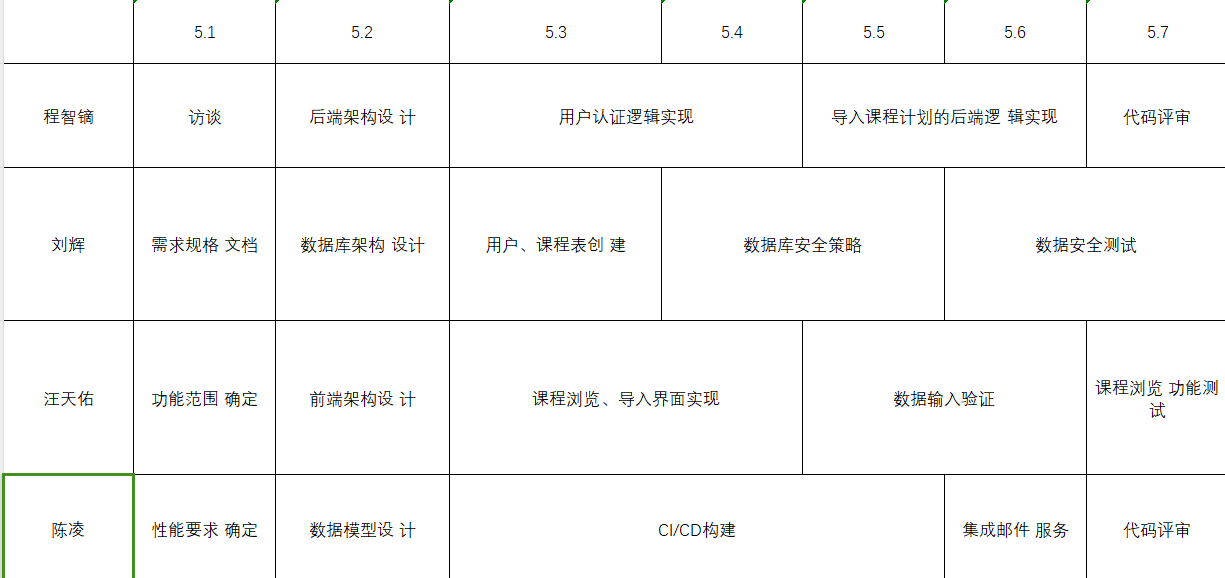
\includegraphics[width=\textwidth]{日程1.png}
	\caption{日程1}
	\label{fig:schedule1}
	\end{figure}
	
	\begin{figure}[h]
	\centering
	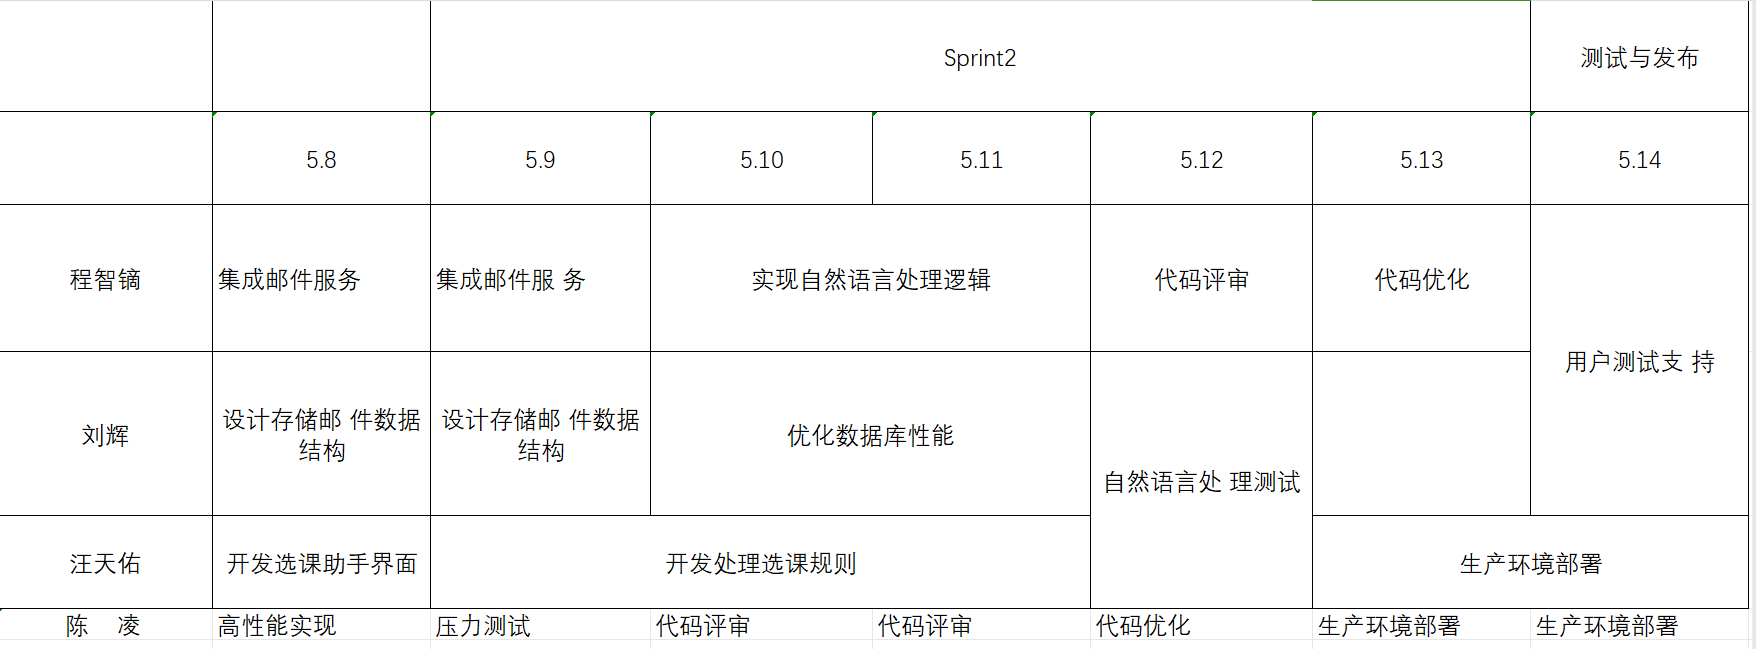
\includegraphics[width=\textwidth]{日程2.png}
	\caption{日程2}
	\label{fig:schedule2}
\end{figure}

\subsection{项目风险管理}
\textbf{技术风险:}
\begin{itemize}
    \item \textbf{风险:} 选择的技术栈可能不够成熟或无法满足系统需求。
    \item \textbf{应对策略:} 在项目前期进行技术评估,验证所选技术的适用性。建立备选方案以备不时之需。
\end{itemize}

\textbf{安全风险:}
\begin{itemize}
    \item \textbf{风险:} 数据泄露、漏洞和未经授权的访问可能导致系统安全问题。
    \item \textbf{应对策略:} 实施强大的身份验证和授权机制,定期进行安全审计和漏洞扫描,及时修复发现的漏洞。
\end{itemize}

\textbf{人员风险:}
\begin{itemize}
    \item \textbf{风险:} 项目团队中的关键成员可能离开或出现能力不足的问题。
    \item \textbf{应对策略:} 确保团队有足够的人员资源,建立知识共享和培训计划,减轻对个别成员的依赖。
\end{itemize}

\textbf{范围风险:}
\begin{itemize}
    \item \textbf{风险:} 需求变更或误解可能导致范围蔓延。
    \item \textbf{应对策略:} 建立严格的变更控制流程,确保每项需求变更都经过评审和批准。与利益相关者进行积极的沟通。
\end{itemize}

\textbf{时间风险:}
\begin{itemize}
    \item \textbf{风险:} 项目进度可能受到延误,导致无法按计划上线。
    \item \textbf{应对策略:} 制定详细的项目计划,设定里程碑并进行定期的进度追踪。提前识别并解决延误问题。
\end{itemize}

\textbf{资源风险:}
\begin{itemize}
    \item \textbf{风险:} 资金、人力和硬件资源可能不足。
    \item \textbf{应对策略:} 在项目启动前进行资源规划,与高层管理层协商项目预算,确保有足够的资源支持项目需求。
\end{itemize}

\textbf{集成和性能风险:}
\begin{itemize}
    \item \textbf{风险:} 不同组件之间的集成问题可能导致系统性能下降或故障。
    \item \textbf{应对策略:} 进行持续的集成测试,确保各个组件协同工作,同时进行性能测试以发现并解决性能问题。
\end{itemize}

\textbf{管理风险:}
\begin{itemize}
    \item \textbf{风险:} 不良的项目管理实践可能导致项目控制失效。
    \item \textbf{应对策略:} 使用有效的项目管理工具和方法,建立明确的沟通渠道,定期审查项目进展。
\end{itemize}

\section{功能特点}

\subsection{登录和用户管理}
\subsubsection{用户注册}
\begin{itemize}
  \item 用户信息收集: 在注册页面,要求用户提供必要的个人信息,如姓名、学号、邮箱地址等。确保用户信息的完整性和准确性。使用表单验证和格式检查,确保数据有效性。
  \item 用户角色选择: 用户在注册时选择其角色,通常分为学生、教师和管理员。每个角色有不同的权限。
  \item 密码安全: 强制要求用户创建强密码,包括字母、数字和特殊字符,并确保密码加密存储。
  \item 邮箱验证: 发送验证邮件到提供的邮箱地址,包括一个唯一的确认链接。用户需要点击确认链接以完成注册。
  \item 防止重复注册: 确保同一邮箱地址或学号不能多次注册。
\end{itemize}

\subsubsection{用户登录}
\begin{itemize}
  \item 用户名密码登录: 用户输入已注册的邮箱地址和密码,系统验证这些信息后允许用户登录。使用多因素认证增加登录操作的安全性和便利性
  \item 记住我: 提供“记住我”选项,以便用户在下次访问时免除重新登录。
  \item 单点登录(可选): 如果系统需要与其他系统集成,可以实施单点登录(SSO)以简化用户登录流程。
\end{itemize}
\subsubsection{角色权限管理}
\begin{itemize}
  \item 角色定义: 定义不同角色的权限,如学生、教师和管理员。每个角色有不同级别的访问和操作权限。
  \item 审计日志: 记录用户的登录和操作,以便审计角色权限的使用情况。
  \item 动态权限管理: 允许管理员根据需要更改角色权限,以反映实际情况, 并且修改应该可以实时生效。
  \item 用户角色切换(如果适用): 如果用户具有多个角色,例如一个教师也可以是学生,实现用户角色切换功能。
  \item 密码重置和账户锁定: 提供密码重置功能,以及在多次登录失败后锁定账户以提高安全性。
  \item 权限分配: 将权限与角色关联,以便更轻松地为用户分配权限。
  \item 角色验证: 在系统的各个部分使用角色验证,确保用户只能执行其具有权限的操作。
\end{itemize}
\subsection{课程管理}
\subsubsection{课程导入}
\begin{itemize}
  \item 灵活性: 系统应具有足够的灵活性,能够处理不同类型的课程,例如公选课,必修课,通识课等等
  \item 数据验证: 在课程导入过程中,进行数据验证,确保课程信息的正确性和完整性。例如,检查每个课程是否包含课程描述、老师等必要信息
\end{itemize}
\subsubsection{课程调整和停止}
\begin{itemize}
  \item 灵活性: 系统应具有足够的灵活性,可以在允许范围内让教师对课程进行任意修改
  \item 兜底限制: 应做好对课程修改的兜底限制,例如: 时间不能调制周末等
\end{itemize}

\subsection{选课策略设置}
\subsubsection{定制化课程参数设置}
\begin{itemize}
  \item 课时设置: 允许管理员或教师根据课程的需要来设定课程的课时. 同时LLM通过提供的数据支持,分析历史课程数据和学生反馈,为课时设置提供智能建议
  \item 考试方式设置: 允许教师根据课程本身的特性和需求来设定课程考核的形式
  \item 选课方式设置: 允许教师根据课程特性设定课程的选课方式,例如:指选,抽签等
\end{itemize}
\subsubsection{学生名单导入}
\begin{itemize}
  \item 数据格式: 允许管理员或教师导入学生名单数据,数据格式可以是常见的 Excel 格式或CSV 格式。
  \item 数据验证: 在导入过程中,进行数据验证,以确保学生名单数据的准确性。例如,检查每个学生是否包括必要的信息,如姓名、学号、班级等。
  \item 批量导入: 支持批量导入,以便一次性导入多个学生名单,减少手动输入的工作量。
  \item 重复数据处理: 处理可能存在的重复数据或重复学生记录,以避免重复导入。
\end{itemize}

\subsection{选课流程}
\subsubsection{自主课程选择}
\begin{itemize}
  \item 选课时间设定: 管理员可以为不同类型的课程设定不同的选课时间
  \item 课程呈现: 在选课开始后,系统应呈现课程列表给同学,以便他们选择课程。
  \item 课程信息预览: 提供教师和学生查看课程信息的功能,以确保选择时可以看见课程的内容。LLM可通过语义理解技术,解析课程信息并生成简洁明了的预览内容。
\end{itemize}

\subsubsection{选课过程支持}
\begin{itemize}
  \item 备选课程展示: 学生应可以对课程加标注,学生可以进行备选课程列表快速选择
  \item 汇总页面: 系统应提供一个汇总页面,显示学生所有选择的课程。这样考生可以了解自己的选课情况。
  \item 超链接导航: 系统应提供超链接,允许学生在不同类型课程之间轻松跳转,并返回到汇总页面。LLM可以优化页面导航,提供个性化的链接推荐,增强用户体验。
\end{itemize}

\subsubsection{防外挂功能}
\begin{itemize}
  \item 反脚本技术: 系统应该做好对学生操作的监控与限流,防止学生使用脚本选课.LLM可以通过行为分析和模式识别,检测和阻止异常选课行为。
  \item 账号锁定: 如果选课期间出现可疑指标,管理员可以远程锁定学生账户,防止进一步作弊。
\end{itemize}

\subsection{智能化体验}
\subsubsection{智能调配}
\begin{itemize}
  \item 课程冲突检测: 系统可以自动检测学生所选择的课程是否存在时间上的冲突,并提供解决方案,如调整课程时间或寻找替代课程。
  \item 课程平衡建议: 基于学生的学业规划和课程安排,系统可以智能地建议学生选择一定比例的核心课程、选修课程和兴趣课程,以保持学业平衡。
\end{itemize}

\subsubsection{实时反馈}
\begin{itemize}
  \item 选课结果预测: 系统可以根据学生的选课情况和历史数据,预测学生最终选择的课程,并提供相应的反馈和建议。
  \item 选课建议优化: 系统可以根据学生的反馈和实际选课结果,不断优化推荐算法,提供更加准确和个性化的选课建议。考虑学生的整体时间管理,提供课外活动和休息时间的优化建议,确保学生在学业和生活之间取得平衡。
\end{itemize}

\subsection*{}
\begin{tabular}{|c|c|c|c|c|c|}
        \hline
        功能模块 & 功能点 & 代码行数 & 累计代码行 & 时间资源 & 累积时间资源(人时) \\
        \hline
        用户登录注册 & 10 & 108 & 108 & 6 & 6\\
        \hline
        权限管理 & 10 & 98 & 196 & 6 & 12 \\
        \hline
        基本UI设计 & 28 & 328 & 524 & 24 & 36 \\
        \hline
        课程管理 & 30 & 350 & 874 & 24 & 60 \\
        \hline
        选课功能 & 45 & 600 & 1474 & 36 & 96 \\
        \hline
        学生名单导入 & 8 & 100 & 1574 & 4 & 100 \\
        \hline
        智能化体验 & 30 & 800 & 2374 & 25 & 125 \\
        \hline
\end{tabular}

\section{用户体验和界面设计}
\subsection{用户友好的界面设计原则}
\begin{itemize}
	\item 简洁明了:各界面设计简单直观,用户可以快速理解和使用。避免使用过多的文字说明,尽量保持布局清晰。
	\item 一致性:在整个选课系统中保持一致的设计风格和元素,各界面的颜色、按钮样式等都需要进行统一。
	\item 个性化:允许用户根据自己的喜好和需求进行一定程度的个性化设置,比如用户可以自主选择选课界面的主题风格。
	\item 易用性:通过合理的导航功能和用户手册来引导用户的功能使用;在用户第一次进入选课界面时通过标签引导用户快速跳转各种课程,快速标记等详细的功能。
\end{itemize}

\subsection{屏幕原型}
\subsubsection{登录界面}
\begin{itemize}
	\item 显示用户名、密码输入框、用户角色选择和登录按钮。
	\item 提供忘记密码的链接或选项。
	\item 设置一个验证码字段以防止机器人登录。
\end{itemize}

\subsubsection{选课界面}
\begin{itemize}
	\item 显示课程列表,每门课程都有课程名、任课教师、上课时间等信息。
	\item 支持查看详情、选择、退选和收藏课程的功能。
	\item 支持选择课程时间范围、课程类别和过滤冲突等功能。
	\item 支持超链接导航,点击后跳转到不同课程。
	\item 提供选课结果按钮,点击后进入选课结果页面。
\end{itemize}

\subsubsection{选课结果页面}
\begin{itemize}
	\item 显示课表,可以按校历查看每周的课程详情。
	\item 支持展示当前课程的总学分、总课时等信息。
	\item 支持超链接导航,点击后跳转到课程详情。
\end{itemize}

\subsubsection{选课助手界面}
\begin{itemize}
	\item 显示助手对话框,提供可选的基础问题列表。
	\item 支持对用户的选课结果进行冲突检测和平衡建议。
	\item 支持管理员的以自然语言交互方式的指令操作。
\end{itemize}

\subsubsection{课程计划管理界面}
\begin{itemize}
	\item 显示课程计划,包含院系、年级等信息。
	\item 支持管理员导入课程计划的按钮,点击后弹出文件选择对话框;提供excel导入模板。
	\item 支持对课程计划进行修改和保存的功能。
\end{itemize}

\subsubsection{课程设置界面}
\begin{itemize}
	\item 显示课程列表,每门课程都有课程信息和课程限制等设置项。
	\item 支持管理员设置课程的目标、内容、教材等课程信息。
	\item 支持管理员设置课程的选择人数上限、先修课程限制等设置。
\end{itemize}

\subsection{用户反馈和改进计划}
\subsubsection{用户反馈渠道}
\begin{itemize}
	\item 在以上界面添加一个意见反馈按钮,当用户点击后可以进入问卷界面,提供的问题可以包括:您认为的缺点,您认为可行的解决方案,您认为可以新添的功能等等。
	\item 在选课完成后,向用户的邮箱发送一封调查问卷,询问用户本次选课的感受,以及您认为可以改进的地方。
\end{itemize}

\subsubsection{改进计划}
\begin{itemize}
	\item 根据用户反馈进行功能改进:根据用户的反馈意见,分析系统存在的问题和不足之处,并针对性地进行功能改进和优化。例如,如果用户普遍反映课程计划导入功能不够灵活的话,可以优化导入模板的设计,增加更多的灵活性选项。
	\item 界面优化和体验改进:根据用户的使用习惯和反馈,对界面进行优化和改进,提升用户体验。例如,如果用户反映选课界面的字体太小难以阅读,可以考虑调整字体大小或增加字体选择选项。
	\item 增加新功能和特性:根据用户需求和市场趋势,考虑增加新的功能和特性来提升系统的吸引力和竞争力。例如,可以考虑添加课程"红黑榜"功能或社交分享功能等。
	\item 定期用户调查和满意度评估:定期开展用户调查和满意度评估活动,了解用户对系统的整体满意度和需求变化,并根据结果制定相应的改进计划。
\end{itemize}

\section{测试和质量保证}
\subsection{测试计划}
\subsubsection{测试类型}
\begin{itemize}
	\item 功能测试:验证系统的各项功能是否按照需求规格说明书的要求正确运行。
	\item 性能测试:评估系统在高负载情况下的性能表现,包括响应时间、吞吐量等指标。
	\item 安全性测试:检查系统的安全性,包括身份验证、权限控制、数据加密等方面。
	\item 兼容性测试:验证系统在不同操作系统、浏览器和设备上的兼容性。
	\item 可用性测试:评估系统的易用性和用户体验,包括界面布局、操作流程等。
	\item 集成测试:验证系统与其他相关系统或组件的集成情况,确保协同工作正常。
\end{itemize}
	
\subsubsection{测试用例}
\begin{itemize}
	\item 功能测试用例:针对每个功能模块设计测试用例,覆盖输入输出的正确性、边界条件、异常处理等。
	\item 性能测试用例:设计不同负载条件下的测试场景,例如同时模拟多个用户进行选课的情况。
	\item 安全性测试用例:包括身份验证、权限控制、数据传输加密等方面的测试用例。
	\item 兼容性测试用例:针对不同操作系统、浏览器和设备进行测试,确保系统在各种环境下正常运行。
	\item 可用性测试用例:设计用户操作流程的测试用例,评估系统的易用性和用户体验。
	\item 集成测试用例:针对与其他系统的接口进行测试,验证数据的传递和交互的正确性。
\end{itemize}

\subsubsection{测试时间表}
\begin{itemize}
	\item 制定详细的测试计划,确定每个阶段的开始和结束日期。
	\item 根据系统的复杂程度和规模,合理分配测试资源和时间。
	\item 将测试阶段划分为单元测试、集成测试、系统测试和验收测试等环节,并设置相应的时间节点。
	\item 根据风险评估的结果,合理安排关键路径上的测试任务。
	\item 跟踪和管理测试进度,及时调整计划以应对可能的变化和问题。
\end{itemize}

\subsection{质量保证计划}
\begin{itemize}
	\item 确定质量目标和标准:明确系统的质量要求和交付标准,并与开发团队成员达成共识。
	\item 设定质量度量指标:设定质量度量指标,追踪和评估项目的质量,确保质量目标的实现。
	\item 制定质量管理计划:明确各个阶段的质量活动和责任分工,确保整个开发过程的质量可控。
	\item 进行代码审查:对系统的源代码进行定期审查,发现潜在问题并提出改进建议。
	\item 完善项目相关文档:确保项目文档的完整性和准确性,提供高质量的文档支持。
	\item 引入自动化测试工具:使用适当的自动化测试工具来提高测试效率和准确性,减少人工错误。
	\item 确保持续集成和持续交付:通过持续集成和持续交付的方式,尽早发现和修复问题,减少后期修改的成本和风险。
	\item 进行性能和安全性测试:定期进行性能和安全性测试,确保系统的稳定性和可靠性。
	\item 进行用户体验测试:邀请真实用户参与系统的使用和评估,收集反馈意见并进行改进
	\item 进行回归测试:在每次发布新版本之前进行回归测试,确保新功能的添加不会对现有功能造成影响。
\end{itemize}

\subsection{A/FR指标计算}
A/FR(Appraisal/Failure Ratio)是软件工程中的一个重要质量指标,用于评估质检成本与失效成本之间的关系。我们对项目的A/FR指标计算如下: \\
1. 质检成本: 设计评审时间 + 代码评审时间 = 24.2 + 57.6 = 81.8人时 \\
2. 失效成本:设计阶段遗留缺陷时间 + 编码阶段遗留缺陷时间 + 代码评审阶段遗留缺陷时间 + 测试阶段遗留缺陷时间 = 14 + 92 + 12 + 5 = 123 人时 \\
3. A/FR指标: A/FR = 81.8/123 = 0.665


\section{部署和维护}
\subsection{部署计划}
\subsubsection{系统上线计划}
\begin{itemize}
	\item 确定上线日期和时间,并与开发团队和运维团队协调好。
	\item 在上线前进行系统测试,确保所有功能正常运行且没有明显的 bug。
	\item 准备上线所需的环境,包括服务器、数据库等。
	\item 将系统部署到生产环境中,并进行相关的配置和初始化操作。
	\item 进行最后的系统检查和验证,确保一切正常。
	\item 通知相关人员和系统用户,告知他们系统已上线并可以开始使用。
\end{itemize}

\subsubsection{环境要求}
\begin{itemize}
	\item 服务器要求:根据系统的负载需求,选择适当的服务器硬件配置,如 CPU、内存、存储空间等。
	\item 操作系统要求:根据系统支持的操作系统版本,选择合适的操作系统。
	\item 数据库要求:根据系统使用的数据库类型,安装和配置相应的数据库服务。
	\item 网络要求:确保服务器与互联网连接畅通,并满足系统的网络带宽要求。
	\item 安全要求:配置防火墙、访问控制等安全措施,保护系统免受未授权访问和攻击。
\end{itemize}

\subsection{维护策略}
\subsubsection{日常维护}
\begin{itemize}
	\item 定期检查服务器和数据库的性能,确保其正常运行并及时处理异常情况。
	\item 监控系统的运行状态和资源利用率,及时发现潜在的性能问题或瓶颈。
	\item 定期备份数据,以防止数据丢失或损坏的情况发生。
	\item 定期更新系统软件和补丁,以修复已知的安全漏洞和提升系统的稳定性。
	\item 定期清理无用的数据和日志文件,释放存储空间并保持系统的良好性能。
	\item 定期维护系统的文档:保持系统的文档处于最新状态,确保文档的准确性和完整性。
\end{itemize}

\subsubsection{升级计划}
\begin{itemize}
	\item 根据业务需求和技术发展,制定系统的升级计划,包括功能扩展、性能优化等方面。
	\item 在升级前进行充分的测试和评估,确保新版本的功能正常且不会对现有系统产生负面影响。
	\item 根据升级计划的时间安排,逐步将新版本部署到生产环境中,并进行相关的数据迁移和回滚策略。
	\item 确保升级过程中的服务可用性,及时通知用户并解决可能出现的问题。
	\item 完成升级后,进行回归测试和性能测试,确认新版本的运行状况和稳定性。
	\item 制定升级后的评估和反馈机制:收集用户反馈,评估升级的效果,并继续进行相应的改进。
\end{itemize}

\section{预算和资源}
\subsection{硬件需求}
\begin{itemize}
	\item 服务器:根据系统的负载需求大概需要两到四台高性能服务器。
	\item 存储设备:预计需要 50TB 的硬盘存储空间。
	\item 网络设备:路由器、交换机等必要的网络设备。
	\item 其他硬件成本:如显示器、键盘、鼠标等。
\end{itemize}

\subsection{软件需求}
\begin{itemize}
	\item 操作系统使用windows 10,无成本。
	\item 数据库管理系统使用开源 MySQL,无授权成本。
	\item 开发工具和集成环境,如 IDEA 的授权费用。
	\item web 服务器和相关中间件,如 redis 等。
\end{itemize}

\subsection{人力资源需求}
\subsubsection{项目团队内部人员}
\begin{itemize}
	\item 项目经理:负责项目的整体规划和管理,内部推举出一人负责。
	\item 开发人员:根据系统的功能需求和开发计划;4 人全部参与,其中一人为开发主负责人,负责需求的统辖和分配。
	\item 测试人员:负责系统测试用例的编写和测试计划的执行;4 人全部参与,其中一人为测试主要负责人。
	\item 运维人员:负责系统的部署和维护工作;选出一人负责,该负责人不是上述提到的项目经理、开发人员和测试人员。
\end{itemize}

\subsubsection{外包团队人员}
考虑到该选课系统需要在 2 周内交付一个产物以赶上本地的选课开始,所以在项目的初期需要投入 4-6 人的外包人力资源来保证产物的交付。

\subsection{成本量化图表}
\begin{figure}[H]
	\centering
	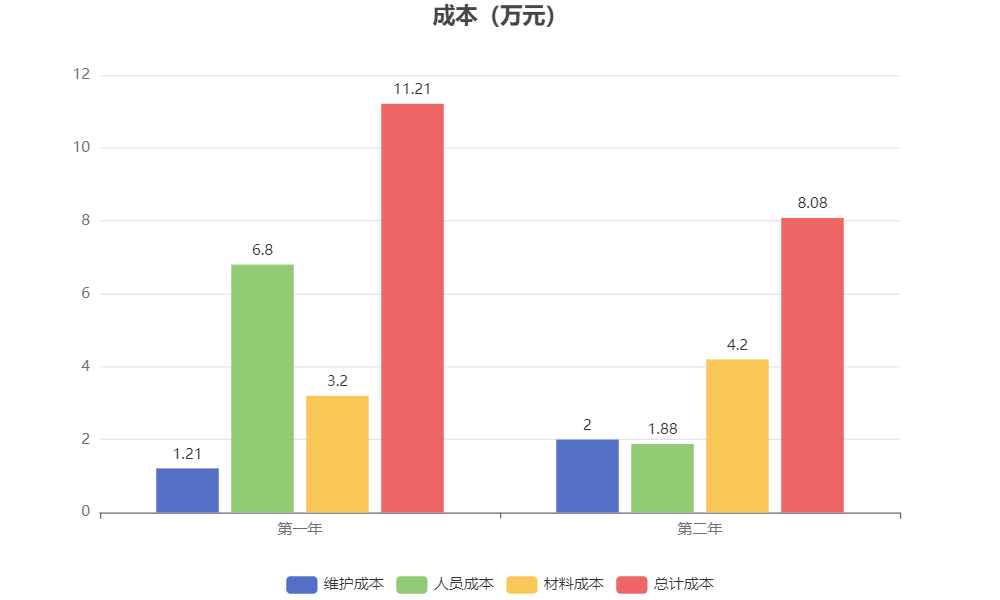
\includegraphics[width=\textwidth]{成本.jpg}
\end{figure}


\section{推进计划}
\begin{itemize}
	\item 项目方案的提交日期:由于 2 周之后本地区会开始选课,赶上该次选课的机会会使系统迅速扩大影响,因此本团队计划在 3 天时间内完成该项目方案的第一阶段设计,并于第三天晚 12:00 前提交项目方案。
	\item 初步产物的交付:如果项目的初步方案通过评审,团队会在两周内交付初版的在线选课系统以来赶上两周后的选课;如果项目方案未能通过评审或者未能及时赶上选课开始,则会按照项目计划表进行原计划的开发与交付。
\end{itemize}

\section{结论}
\subsection{项目核心要点}
\begin{itemize}
	\item 灵活的课程计划导入功能:用户能够将课程计划以 Excel 表格的形式批量导入,并支持不同院系和不同年级同时导入。
	\item 严格的防脚本措施:系统能够对用户操作进行监控与限流,确保选课的公平性和安全性。
	\item 自动生成课表:系统能够根据用户的选课结果自动生成课表,并提供冲突监测和平衡分析功能,方便用户评估自己的选课情况。
	\item LLM助手:系统能够使用大语言模型为用户提供周到的引导服务和基于自然语言的指令操作。
	\item 权限管理与角色分配:系统支持不同角色的选课权限和课程设置等资源的权限控制,确保数据的安全性和完整性。
	\item 高度可定制性:系统提供了丰富的 API 接口和插件机制,便于其他开发者进行个性化的功能扩展和定制需求。
	\item 多语言支持:系统支持多种语言界面,方便不同地区的用户参与在线选课。
	\item 数据备份与恢复:系统能够定期进行数据备份,并提供数据恢复功能,保障选课信息课程信息等数据的安全性和可靠性。
\end{itemize}

\subsection{潜在价值}
\begin{itemize}
	\item 提升选课效率:通过在线选课系统,学生可以随时随地参加选课,无需安排时间和地点,大大节省了时间和人力资源成本。同时,系统的自动生成课表和选课助手功能也提高了选课的效率。
	\item 增加选课公平性:系统的防脚本措施可以有效防止使用脚本抢课行为的发生,保证了选课的公平性和公正性。
	\item 提供数据分析与反馈:系统提供的课表分析功能可以帮助用户更好地了解自己的选课情况,及时调整选课策略。
	\item 拓展教育资源:在线选课系统可以为教育行业提供更广泛的资源利用和共享平台,使得教育机构能够更加便捷地管理选课任务,提高教学质量和效果。
\end{itemize}

\end{document}
